\documentclass[tikz]{standalone}
\usetikzlibrary{decorations.markings}
\begin{document}
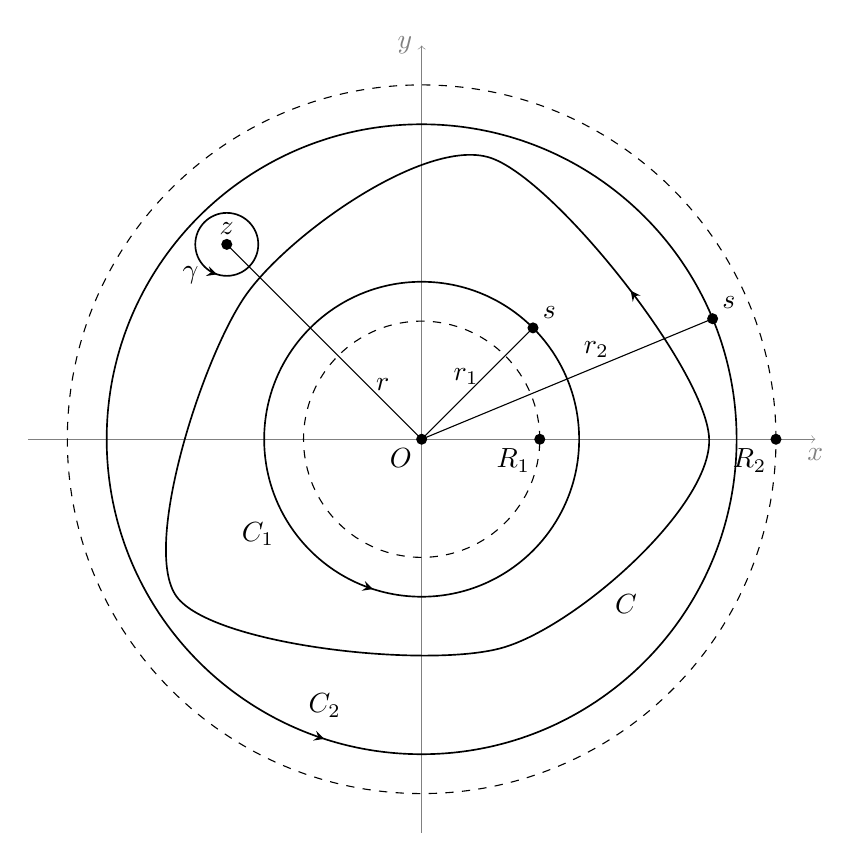
\begin{tikzpicture}[decoration={
    markings,% switch on markings
    mark=at position 0.7 with {\arrow{stealth}},
  }]

  % Draw axes with labels
  \draw [help lines, ->] (-5,0) -- (5,0) node [below] {$x$};
  \draw [help lines, ->] (0,-5) -- (0,5) node [left] {$y$};

  % Define coordinates first
  \coordinate [label=below left:$O$] (O) at (0,0);
  \fill (O) circle (2pt);
  \coordinate [label=below left:$R_1$] (R1) at (1.5,0);
  \fill (R1) circle (2pt);
  \coordinate [label=below left:$R_2$] (R2) at (4.5,0);
  \fill (R2) circle (2pt);
  \coordinate [label=above right:$s$] (s1) at (45:2);
  \fill (s1) circle (2pt);
  \coordinate [label=above right:$s$] (s2) at (22.5:4);
  \fill (s2) circle (2pt);
  \coordinate [label=above right:$C$] (c) at (315:3.3);
  \coordinate [label=above:$z$] (z) at (135:3.5);
  \fill (z) circle (2pt);

  % Draw circles
  \draw[style=dashed] (O) circle (1.5);
  \draw[style=dashed] (O) circle (4.5);
  \draw[postaction={decorate}, line width=0.6pt] (O) circle (2) ++(210:2.4) node {$C_1$};
  \draw[postaction={decorate}, line width=0.6pt] (O) circle (4) ++(250:3.6) node {$C_2$};
  \draw[postaction={decorate}, line width=0.6pt] (z) circle (0.4) ++(220:0.6) node {$\gamma$};

  % random closed curve
  \pgfmathsetseed{4}
  \draw[postaction={decorate}, line width=0.6pt] plot [smooth cycle, samples=5,domain={1:5}]
  (\x*360/5:2.5+1.5*rnd);

  % Mark radi
  \path[draw] (O) -- (s1) node[pos=0.4, above] {$r_1$};
  \path[draw] (O) -- (s2) node[pos=0.6, above] {$r_2$};
  \path[draw] (O) -- (z) node[pos=0.2, above] {$r$};
\end{tikzpicture}
\end{document}
